\documentclass[paperwidth=841mm,paperheight=1189mm,portrait]{baposter}
%\documentclass[portrait,a0,final]{baposter}
\usepackage{caption}
\usepackage{booktabs}
\usepackage{wrapfig}
\usepackage{lmodern}
\usepackage{paralist}
\usepackage{authblk}
\usepackage[utf8]{inputenc} %unicode support
\usepackage[T1]{fontenc}
\usepackage{tabularx}
\usepackage{amsmath,amssymb}
\usepackage[numbers,square,sort&compress]{natbib}
\renewcommand{\bibsection}{}

\selectcolormodel{cmyk}

\graphicspath{{figures/}} % Directory in which figures are stored


\newcommand{\compresslist}{%
\setlength{\itemsep}{0pt}%
\setlength{\parskip}{1pt}%
\setlength{\parsep}{0pt}%
}

\newenvironment{boenumerate}
  {\begin{enumerate}\renewcommand\labelenumi{\textbf\theenumi.}}
  {\end{enumerate}}



\begin{document}


\definecolor{darkgreen}{cmyk}{0.8,0,0.8,0.45}
\definecolor{lightgreen}{cmyk}{0.8,0,0.8,0.25}
\definecolor{redbitdefender}{cmyk}{0,1,1,0.2}
\definecolor{blackbitdefender}{cmyk}{1,1,1,1}

\begin{poster}
{
grid=false,
headerborder=open, % Adds a border around the header of content boxes
colspacing=2em, % Column spacing
bgColorOne=white, % Background color for the gradient on the left side of the poster
bgColorTwo=white, % Background color for the gradient on the right side of the poster
borderColor=blackbitdefender, % Border color
headerColorOne=redbitdefender, % Background color for the header in the content boxes (left side)
headerColorTwo=redbitdefender, % Background color for the header in the content boxes (right side)
headerFontColor=white, % Text color for the header text in the content boxes
boxColorOne=white, % Background color of the content boxes
textborder=rounded, %rectangle, % Format of the border around content boxes, can be: none, bars, coils, triangles, rectangle, rounded, roundedsmall, roundedright or faded
eyecatcher=false, % Set to false for ignoring the left logo in the title and move the title left
headerheight=0.12\textheight, % Height of the header
headershape=rounded, % Specify the rounded corner in the content box headers, can be: rectangle, small-rounded, roundedright, roundedleft or rounded
headershade=plain,
headerfont=\Large\textsf, % Large, bold and sans serif font in the headers of content boxes
%textfont={\setlength{\parindent}{1.5em}}, % Uncomment for paragraph indentation
linewidth=0.25pt % Width of the border lines around content boxes
}
{}
%
%----------------------------------------------------------------------------------------
%	TITLE AND AUTHOR NAME
%----------------------------------------------------------------------------------------
%
{
\textsf %Sans Serif
{Continual Learning with O-LoRA: Orthogonal Low-Rank Adapters for Sequential Tasks}
}
{\sf\vspace{0.1em}\\
Alex Birsan, Radu Savin
\vspace{0.1em}\\
\small{University of Bucharest, Romania}
}
{\IfFileExists{figures/unibuc.png}{
\includegraphics[scale=0.5]{unibuc}}{\fbox{\parbox[c][3cm][c]{5cm}{\centering\sf University\\of Bucharest}}}} % University/lab logo


\headerbox{1. Introduction}{name=problem,column=0,span=1}{

Continual learning requires a model to sequentially acquire knowledge across multiple tasks
without forgetting what it previously learned. A common challenge is \textbf{catastrophic
forgetting}: adapting to a new task overwrites representations built for earlier ones.

When parameter-efficient methods such as \textbf{LoRA}~\citep{Hu2022LoRA} are applied in this setting, the
low-rank adapter matrices trained on successive tasks tend to occupy overlapping subspaces,
causing destructive interference.

\textbf{O-LoRA}~\citep{Wang2023OLoRA} addresses this by imposing an orthogonality constraint
on the $A$ matrices of each new task adapter with respect to all previously learned ones,
ensuring each task projects inputs into a distinct region of the low-rank latent space and
limiting the interference that drives forgetting.

}

\headerbox{2. Dataset and Preprocessing}{name=sketch,column=0,below=problem,span=1}{

\textbf{Task sequence (fixed order):}
\begin{compactitem}
  \item \textbf{AG News}~\citep{Zhang2015CharCNN} -- 4-class news topic classification
  \item \textbf{Amazon Polarity}~\citep{McAuley2015} -- binary sentiment classification
  \item \textbf{DBpedia 14}~\citep{Zhang2015CharCNN} -- 14-class Wikipedia topic classification
  \item \textbf{Yahoo Answers Topics}~\citep{Zhang2015CharCNN} -- 10-class question topics
\end{compactitem}
Each task is trained on independently, with no replay of prior task data.

\textbf{Instruction-tuning prompt format:}
\begin{center}\small
\begin{tabular}{l}
\toprule
\texttt{\{task instruction\}\textbackslash n}\\
\texttt{Option: \{comma-separated label names\}\textbackslash n}\\
\texttt{\{input text\}\textbackslash n}\\
\texttt{Answer:}\\
\bottomrule
\end{tabular}
\end{center}
Only the input text is truncated when the sequence exceeds the maximum length. Cross-entropy
loss is computed only on the label token; at evaluation the predicted label is the candidate
label token with maximum logit at the position before \texttt{Answer}.

}




\headerbox{3. Models}{name=architecture,span=2,column=1}{

\textbf{Backbone:} Qwen2.5-1.5B~\citep{Qwen2024}.\hspace{2em}
\textbf{LoRA adapters:} rank $r=8$, scaling $\alpha=32$, dropout 0.1, applied to the query and
value projections of every attention layer.\hspace{2em}
\textbf{Optimisation:} 1 epoch / task, learning rate $10^{-3}$, batch size 8.

\vspace{0.4em}
\textbf{Compared methods:}
\begin{compactitem}
  \item \textbf{IncLoRA} -- interference-free upper bound: a separate adapter trained
        and frozen for each task ($\text{BWT}=0$ by construction~\citep{LopezPaz2017GEM}).
  \item \textbf{O-LoRA} -- a single cumulative adapter penalising overlap between the new
        task's $A$ matrix and all previously learned ones via an orthogonal regularisation
        term weighted by $\lambda_1 \in [0.2, 0.3]$.
\end{compactitem}

\vspace{0.4em}
\textbf{Orthogonal loss.} For task $t$ with adapter $\Delta W_t = B_t A_t$:
\[
\mathcal{L}_t \;=\; \mathcal{L}_{\mathrm{CE}}(A_t,B_t)
\;+\; \lambda_1 \!\!\sum_{i<t}\bigl\lVert A_t A_i^{\!\top}\bigr\rVert_F^{2}
\]
The penalty drives the row-spaces of successive $A$ matrices into mutually orthogonal
directions. Crucially, \textbf{no constraint is applied to the $B$ matrices}.

}


\headerbox{4. Results}{name=res,column=1,below=architecture,span=2}{

\noindent
\begin{tabular}[t]{@{}l@{\hspace{1.2cm}}l@{}}
\begin{tabular}[t]{lc}
\multicolumn{2}{l}{\textbf{IncLoRA baseline (no forgetting):}}\\
\toprule
\textbf{Task} & \textbf{Accuracy}\\
\midrule
AG News              & 0.854\\
Amazon Polarity      & 0.956\\
DBpedia 14           & 0.972\\
Yahoo Answers Topics & 0.640\\
\bottomrule
\end{tabular}
&
\begin{tabular}[t]{lcc}
\multicolumn{3}{l}{\textbf{Impact of prompt structure:}}\\
\toprule
\textbf{Prompt format} & \textbf{Avg Acc} & \textbf{BWT}\\
\midrule
Old (no label options)      & 0.597 & $-0.344$\\
New (instruction + options) & 0.799 & $-0.091$\\
\bottomrule
\end{tabular}
\end{tabular}

\vspace{0.8em}
\textbf{O-LoRA -- summary metrics:}\\[2pt]
\begin{tabular}{lcccc}
\toprule
\textbf{Run} & \textbf{Samples / task} & $\boldsymbol{\lambda_1}$ & \textbf{Avg Acc} & \textbf{BWT}\\
\midrule
Short             & 500/500/500/500     & 0.3 & 0.846 & $-0.032$\\
2h                & 500/650/1850/1300   & 0.2 & 0.799 & $-0.091$\\
Full ($\sim$50\%) & 2100/2700/7500/5300 & 0.3 & 0.654 & $-0.268$\\
\bottomrule
\end{tabular}

\vspace{0.4em}
\textbf{Per-task accuracy: initial $\rightarrow$ final}\\[2pt]
\small
\begin{tabular}{lccc}
\toprule
\textbf{Task} & \textbf{Short} & \textbf{2h} & \textbf{Full ($\sim$50\%)}\\
\midrule
AG News              & 0.878$\to$0.825 ($-6\%$)    & 0.842$\to$0.747 ($-11\%$) & 0.887$\to$0.494 ($-44\%$)\\
Amazon Polarity      & 0.956$\to$0.957 ($\sim$0\%) & 0.947$\to$0.915 ($-3\%$)  & 0.905$\to$0.746 ($-18\%$)\\
DBpedia 14           & 0.964$\to$0.919 ($-5\%$)    & 0.979$\to$0.833 ($-15\%$) & 0.980$\to$0.729 ($-26\%$)\\
Yahoo Answers Topics & 0.683$\to$0.683 (---)       & 0.702$\to$0.702 (---)     & 0.649$\to$0.649 (---)\\
\bottomrule
\end{tabular}\\[2pt]
\normalsize
Avg accuracy and BWT both \textbf{degrade as the number of training samples grows}, even
though more data improves \emph{initial} per-task accuracy. The \textbf{instruction + options}
prompt format yields $+0.20$ Avg Acc and $+0.25$ BWT -- a larger effect than any
hyperparameter choice.

\vspace{0.3em}
\begin{center}
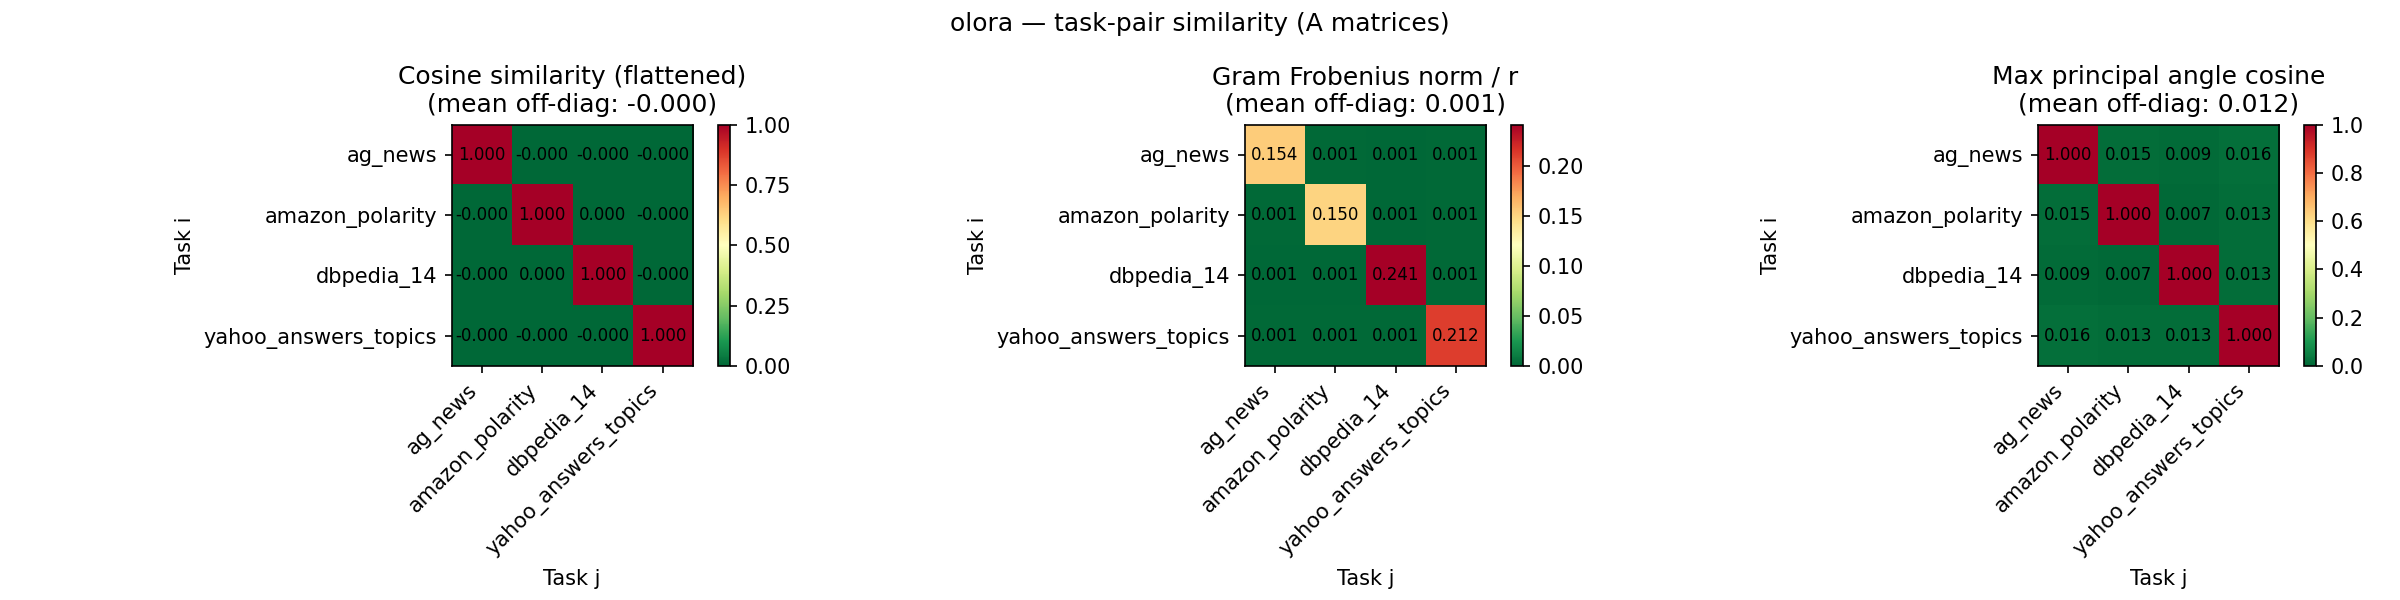
\includegraphics[width=0.55\textwidth]{task_similarity_A.png}\\
{\footnotesize Pairwise similarity of $A$ matrices: cosine, Gram Frobenius norm $/r$,
max principal angle cosine -- all near-zero off-diagonal.}
\end{center}

\vspace{0.1em}
\textbf{Orthogonality analysis.} All three metrics show near-zero similarity across $A$ even
with $\lambda_1 \in [0.2,0.3]$ -- the constraint is easy to satisfy. However $B$ matrices,
unconstrained by the loss, share $\sim 30\%$ of their column-space directions
(principal-angle cosine $\sim 0.29$) and grow in magnitude with training -- plausibly the
primary driver of forgetting at higher scales.

}


\headerbox{6. References}{name=refs,column=0,above=bottom,span=1}{
\renewcommand{\section}[2]{}%
\scriptsize
\bibliographystyle{plainnat}
\bibliography{poster}
}

\headerbox{5. Conclusion}{name=conclusion,column=1,below=res,span=2}{
\begin{compactitem}
  \item O-LoRA's regulariser keeps $A$ matrices \textbf{geometrically separated} with mild
        penalties; translating this into reduced forgetting is \textbf{highly sensitive to
        data scale} -- near-zero BWT at 500 samples/task, sharp collapse ($-0.268$) at
        $\sim$50\% of the paper's scale.
  \item The unregularised $B$ matrices grow in magnitude and share $\sim 30\%$ of their
        column-space directions across tasks -- a likely primary driver of forgetting at scale.
  \item \textbf{Prompt structure matters more than hyperparameters}: explicitly listing label
        names yields $+0.20$ accuracy and $+0.25$ BWT.
\end{compactitem}
}


\end{poster}

\end{document}
